\documentclass[10pt,a4paper]{article}
\usepackage[margin=2.2cm]{geometry}
\usepackage{fontspec}
\usepackage{kotex}
\setmainfont{Apple SD Gothic Neo}
\setsansfont{Apple SD Gothic Neo}
\usepackage{amsmath,amssymb}
\usepackage{graphicx}
\usepackage{booktabs}
\usepackage{caption}
\usepackage[dvipsnames]{xcolor}
\usepackage[colorlinks=true,linkcolor=MidnightBlue,citecolor=MidnightBlue,
            urlcolor=MidnightBlue]{hyperref}
\usepackage{titlesec}
\titleformat{\section}{\large\bfseries}{\thesection}{0.6em}{}
\titleformat{\subsection}{\normalsize\bfseries}{\thesubsection}{0.5em}{}
\captionsetup{font=small,labelfont=bf}
\setlength{\parskip}{0.35em}
\setlength{\parindent}{0pt}

\usepackage{mdframed}
\newmdenv[linewidth=0.4pt,linecolor=gray!60,backgroundcolor=gray!5,
          innertopmargin=6pt,innerbottommargin=6pt,skipabove=8pt,skipbelow=8pt]{claimbox}
\newcommand{\claim}[2]{\begin{claimbox}\textbf{주장.} #1\par\smallskip
  \textcolor{gray!70}{\textbf{반증 조건.} #2}\end{claimbox}}

\title{\bfseries 해롭다는 갈래가 없었다\\[2pt]
\large 게임과 도서의 마지막 열 --- 그리고 세 번째 규칙 구멍}
\author{월드모델 실험실 · 노트 $799$}
\date{2026-08-07}
\begin{document}\maketitle

\section{한 줄}

논문 $155$ 가 미결로 남긴 반증 조건을 시험했다 --- \emph{``게임·도서에 $1$열만
넣으면 얇은 도메인 비용이 줄고, 그때도 못 넘으면 두께가 아니라 내용이다.''}

열은 \textbf{결과 무관 규칙}(값 가짓수 최다)이 골랐다: 게임 \texttt{gm\_ndlc}
(DLC 수 · $55$값) · 도서 \texttt{bk\_weight}(무게 · 내 예상은 쪽수였는데 규칙이
무게를 골랐다 --- 규칙이 고르는 것이 맞다).

\textbf{게임은 미달}($+0.0123 < 2\sigma\ 0.0195$)이고 \textbf{도서는 해롭다}
($-0.1071$ · 위약 여섯 전부보다 낮음). 두 갈래 다 닫는다. 그리고 도서의 결과는
\textbf{내 사전등록 갈래 어디에도 안 들었다} --- 세 번째 규칙 구멍이고, 이번에는
규약($45$)으로 세웠다.

\begin{figure}[t]\centering
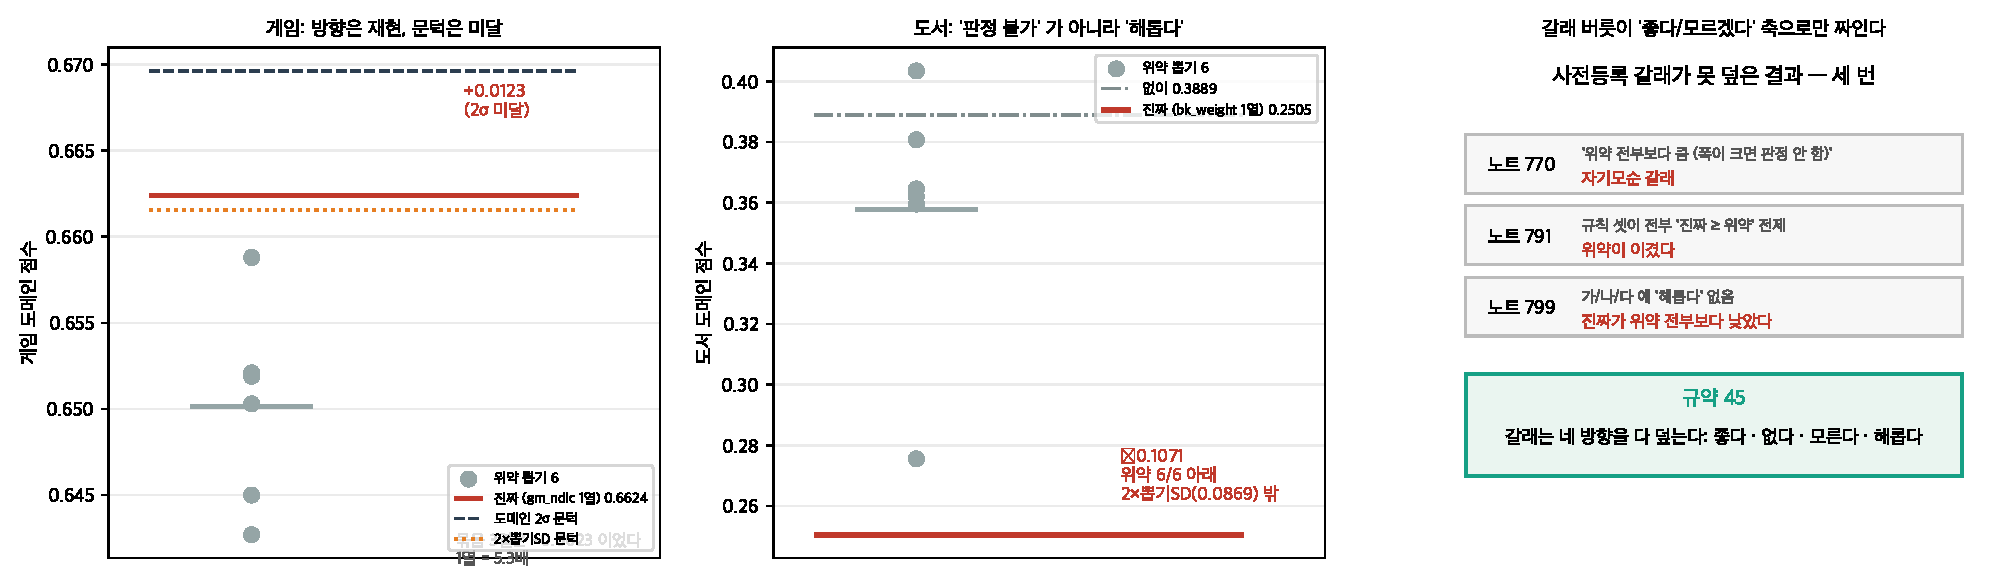
\includegraphics[width=0.99\textwidth]{figs/harm.pdf}
\caption{왼쪽: 게임 --- 위약 $6/6$ 과 $2\times$뽑기SD 는 넘고 $2\sigma$ 는 미달.
가운데: 도서 --- 진짜가 위약 여섯 \textbf{전부보다} 낮다. 오른쪽: 같은 꼴의 규칙
구멍 세 번.}
\end{figure}

\section{게임 --- 방향은 재현되고 문턱은 미달}

\begin{center}
\begin{tabular}{lrl}
\toprule
없이(게임 점수) & $0.6586$ & \\
\textbf{진짜}(\texttt{gm\_ndlc} $1$열) & $\mathbf{0.6624}$ & \\
위약 뽑기 $6$ & 평균 $0.6501$ · SD $0.0057$ & \\
\midrule
신호 몫 & $\mathbf{+0.0123}$ & \\
$2\times$뽑기SD & $0.0114$ & 넘는다 \\
위약 전부보다 큼 & $6/6$ & 넘는다 \\
\textbf{도메인 $2\sigma$} & $0.0195$ & \textcolor{BrickRed}{\textbf{미달}} \\
\bottomrule
\end{tabular}
\end{center}

\claim{\textbf{열 절제 효과는 게임에서도 방향이 재현된다.} 묶음 $3$열이 $+0.0023$
이었고 $1$열이 $\mathbf{+0.0123}$ --- $5.3$배다. 만화($0.0231 \to 0.0272$)에 이어
두 번째 도메인이다. \textbf{그러나 사전등록 (나)가 발동한다} --- 게임 유보 $180$행의
표본 $2\sigma$(0.0195)가 신호보다 크다. \textbf{갈래를 닫는다.}}
{이것은 ``신호가 없다''가 아니라 \textbf{``이 표본으로는 못 가른다''}다. 게임
유보가 $2.5$배(약 $450$행) 자라면 $2\sigma$ 가 $0.0123$ 아래로 내려와 지금 신호로
판정이 선다 --- 다시 꺼낼 조건으로 적는다. \textbf{행을 늘리는 것이 모델을 만지는
것보다 검출력이 크다는 다섯 번째 사례다.}}

\section{도서 --- ``판정 불가''가 아니라 ``해롭다''}

\begin{center}
\begin{tabular}{lrl}
\toprule
없이(도서 점수) & $0.3889$ & \\
\textbf{진짜}(\texttt{bk\_weight} $1$열) & $\mathbf{0.2505}$ & \\
위약 뽑기 $6$ & $0.2755 \sim 0.4034$ · 평균 $0.3576$ & \\
\midrule
신호 몫 & $\mathbf{-0.1071}$ & $2\sigma$($0.0205$)의 $5$배 \\
$2\times$뽑기SD & $0.0869$ & \textbf{그것도 넘는다} \\
위약과의 자리 & \textcolor{BrickRed}{\textbf{여섯 전부보다 낮다}} & \\
판 변화 & $-0.0081$ & \\
\bottomrule
\end{tabular}
\end{center}

\claim{\textbf{진짜 열이 무작위 값보다 뚜렷이 해롭다.} 논문 $155$ 의 도서
``판정 불가''(위약 폭이 신호를 삼킴)는 이 $1$열에서 \textbf{``해롭다''로 올라간다}
--- 학습 $80$행에서 배운 무게-라벨 관계가 유보 $163$행에서 반대로 작동한다
(과적합인지 시간 드리프트인지는 안 갈랐다). 도서 갈래를 닫고 학습 행 $3$배($240$)
조건만 남긴다. \textbf{그리고 해로운 열은 도메인 몫보다 크게 판을 깎는다} ---
도서는 판의 $1.1\%$($243$행)인데 판을 $-0.0081$ 움직였다. 노트 $646$ 의 ``작은
도메인은 판을 못 움직인다''는 \textbf{이로운 쪽 한정}이었다.}
{내 예측 ②는 ``판정 불가 재현 확률 절반''이었다 --- \textbf{반만 맞았다.} 뽑기
SD 는 크지만($0.0435$) 결과는 그 잡음 \emph{밖에서} 해로웠다. 위약 폭이 큰
도메인에서도 충분히 큰 효과는 갈린다 --- ``얇은 도메인 = 판정 불가''를 공식처럼
쓰면 안 된다.}

\subsection*{세 번째 규칙 구멍 --- 규약 $45$}

내 갈래는 셋이었다: (가) 넘음 · (나) $|$신호$| < 2\sigma$ · (다) 뽑기 SD 가 커서
판정 불가. \textbf{실측($-0.1071$ · 판정 가능한 해로움)은 어디에도 안 든다.}

\claim{\textbf{같은 꼴로 세 번째다} --- 노트 $770$(자기모순 갈래) · $791$(위약이
이기는 경우 없음) · $799$(해로운 경우 없음). \textbf{내 갈래 버릇이
``좋다/모르겠다'' 축으로만 짜인다.} 규약 $45$: \emph{결정 규칙은 네 방향을 다
덮는다 --- 좋다 · 없다 · 모른다 · 해롭다.}}
{이 규약은 자동 검사가 어렵다(산문이라). `check` 가 못 지키는 규약은 사람 기억에
기대는 규약이고, 이 저장소에서 그런 규약의 생존율은 낮았다 --- \textbf{다음
사전등록 몇 개에서 실제로 지켜지는지가 시험이다.}}

\section{T$4$ 의 자리}

원천 열 갈래가 이것으로 정리됐다: 만화 \textbf{통과·서랍}(집 밖 $0.0002$ 미달) ·
게임 \textbf{미달·닫음}(행 부족) · 도서 \textbf{해로움·닫음}. 남는 길은 전부
\textbf{수집}이다 --- KR 짝의 자연 성장, 새 집 밖 짝, 두꺼운 도메인의 후보 열.
다섯 트랙째 같은 곳을 가리킨다.

\end{document}
